\vspace{1cm}
\fancyhead[C]{\normalsize\textbf{$\qquad$ Teil I: Offene Aufgaben}}
\renewcommand{\labelenumi}{\theenumi.}
\section*{Aufgabe 1 (38 Punkte)}
\vspace{0.4cm}
%\titleformat{\subsection}[runin]
%{\normalfont\large\bfseries}{\thesubsection}{1em}{}
\subsection*{\aufgabe{a1}{8}} 
Die Wirtschaftsredakteurin eines wichtigen Verlagshauses zieht in Betracht,
kostenlose Exemplare eines Buchs an Dozierende der Wirtschaftswissenschaften an Schweizer Hochschulen zu verschicken, da sie weiss, dass Dozierende dazu neigen, Bücher als Kurslektüre auszuwählen, die sie bereits in ihren Regalen stehen haben. Die Fixkosten dieser Werbekampagne belaufen sich auf $100'000$ Schweizer Franken.
Die Stückkosten eines einzelnen Buchs betragen $10$ Schweizer Franken, im Handel werden die Bücher schließlich für $40$ Schweizer Franken pro Exemplar verkauft.
Auf der Basis historischer Daten schätzt die Redakteurin, dass wenn $x$ Gratisexemplare versendet werden, ein Verkauf von insgesamt
\begin{align*}
	B(x) = 20'000 - 19'000 e^{-0.0002 x }
\end{align*}
Exemplaren des Buchs erzielt wird. \\
\\
Zeigen Sie, dass wenn die Produktion auf maximal $6'000$ Bücher beschränkt ist, es genau eine Menge $ x^\star \in (0, 6'000)$ an Gratisexemplaren gibt, bei der die Gesamtkosten genau durch den Umsatz gedeckt werden.
\
\\ \\
\textbf{Lösung:}
\begin{mdframed}
\underline{\textbf{Vorgehensweise:}}
\renewcommand{\labelenumi}{\theenumi.}
\begin{enumerate}
\item 

\end{enumerate}
\end{mdframed}
\underline{1. }\\

 
\newpage

\subsection*{\aufgabe{a2}{8}}
Die Wirtschaftsredakteurin eines wichtigen Verlagshauses zieht in Betracht,
kostenlose Exemplare eines Buchs an Dozierende der Wirtschaftswissenschaften an Schweizer Hochschulen zu verschicken, da sie weiss, dass Dozierende dazu neigen, Bücher als Kurslektüre auszuwählen, die sie bereits in ihren Regalen stehen haben. Die Fixkosten dieser Werbekampagne belaufen sich auf $100'000$ Schweizer Franken.
Die Stückkosten eines einzelnen Buchs betragen $10$ Schweizer Franken, im Handel werden die Bücher schließlich für $40$ Schweizer Franken pro Exemplar verkauft.
Auf der Basis historischer Daten schätzt die Redakteurin, dass wenn $x$ Gratisexemplare versendet werden, ein Verkauf von insgesamt
\begin{align*}
	B(x) = 20'000 - 19'000 e^{-0.0002 x }
\end{align*}
Exemplaren des Buchs erzielt wird. Wenn die Produktion auf maximal $6'000$ Bücher beschränkt ist, gibt es genau eine Menge $ x^\star \in (0, 6'000)$ an Gratisexemplaren, bei der die Gesamtkosten genau durch den Umsatz gedeckt werden.\\
\\
Verwenden Sie eine Taylor-Approximation zweiter Ordnung im Punkt $x_0 = 750$, um eine Näherung für $x^\star$ zu finden.
\\
 \\
\textbf{Lösung:}
\begin{mdframed}
\underline{\textbf{Vorgehensweise:}}
\renewcommand{\labelenumi}{\theenumi.}
\begin{enumerate}
\item Bestimme das Taylorpolynom. 
\end{enumerate}
\end{mdframed}

\underline{1. Bestimme das Taylorpolynom}\\

\newpage
\subsection*{\aufgabe{b}{12}}
Anne und Robert haben gerade erfolgreich ihr Masterprogramm in Quantitativen
Methoden an der Universität St.Gallen abgeschlossen und sind nun dabei, ihre eigene
Firma AlgoTrade aufzubauen, die Machine Learning Algorithmen für den computergesteuerten Handel an Finanzmärkten entwickelt. Sie haben bereits viele vielversprechende Ideen, jedoch fehlt ihnen das Eigenkapital. Die anfänglichen Investitionen für den Kauf der IT-Infrastruktur und für die Entwicklung der Software belaufen sich auf $1'500'000$ Schweizer Franken.
Ein Risikokapitalgeber ist zu einem Investment in Höhe von $500'000$ Schweizer Franken bereit, verlangt aber im Gegenzug einen Anteil von $30 \%$ an der Firma.
Zusätzlich nehmen Anne und Robert am 1. Januar 2022 einen Kredit in Höhe von $1'000'000$ Schweizer Franken zu einem jährlichen Zinssatz von $2 \% $ auf.
Die Bank verlangt dabei, dass $40 \%$ des geschuldeten Betrags bis Ende 2026 über konstante Zahlungen $C$, fällig jeweils am Jahresende, zurückgezahlt sein muss.
\begin{enumerate}
	\item[(b1)] Fügen Sie die Ereignisse und Mittelflüsse dem Zeitstrahl hinzu.
	\item[(b2)] Berechnen Sie die Höhe der Ratenzahlung $C$.
\end{enumerate}
Bereits nach 3 Jahren ist AlgoTrade sehr erfolgreich und generiert beträchtliche Umsätze. Beginnend mit der nächsten Rückzahlung am 31. Dezember 2025 wollen Anne und Robert jeweils $180'000$ Schweizer Franken am Ende jedes Jahres solange zurückzahlen, bis die bestehende Restschuld komplett getilgt ist.
\begin{enumerate}
	\item[(b3)] Ergänzen Sie die Information am Zeitstrahl und berechnen Sie die Restschuld am 1. Januar 2025, also direkt nach der jüngsten Rückzahlung.
	\item[(b4)] Am 1. Januar 2029, direkt nach der jüngsten Rückzahlung, verkaufen Anne und Robert	ihre Firma für $5'000'000$ Schweizer Franken und tilgen mit ihrem Anteil die bestehende	Restschuld. Wie hoch ist ihr Gewinn?
\end{enumerate}
\begin{center}
	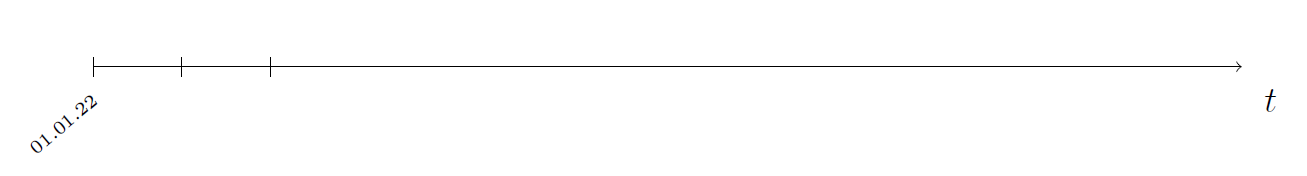
\includegraphics[scale=0.45]{pictures/zeitstrahl_1_b}
\end{center}
\ \\
\textbf{Lösung:}
\begin{mdframed}
\underline{\textbf{Vorgehensweise:}}
\begin{enumerate}
\item[(b1)] Füge den Kredit und die Raten zum Zeitstrahl hinzu.
\end{enumerate}
\end{mdframed}

\underline{(b1) }\\


\newpage
\subsection*{\aufgabe{c}{10}}
Information spielt in der Entscheidungsfindung eine wesentliche Rolle. Allerdings
sehen sich Unternehmen, wie wir erst kürzlich beobachten konnten, einem Zielkonflikt
ausgesetzt. Einerseits ermöglicht das Sammeln möglichst genauer privater Informationen eine verbesserte, massgeschneiderte Lösung für ihre Kunden (die zu einem höheren Preis verkauft werden kann), andererseits erhöht es den potentiellen Schaden, den sie ihren Kunden durch Datenschutzverletzungen (und sich selbst durch mögliche juristische Folgen) zufügen könnten.\\
\\
Sei $I \geq 0 $ die Menge an Informationen, die ein Unternehmen sammelt, und $b(I)$ der Nutzen für den Kunden hinsichtlich der angebotenen Dienstleistung oder des angebotenen Produktes. Wir nehmen an, dass:
\begin{align*}
	b(I)
	= 
	\begin{cases}
		0 &\quad \textrm{für } 0 \leq I  < I_0\\
		s \left( 1 - \frac{I_0}{I} \right) & \quad \textrm{für } I \geq I_0
	\end{cases}.
\end{align*}
Demnach ist $I_0 > 0 $ die Mindestmenge an Information, die benötigt wird, um einen Nutzen für den Kunden zu generieren, und der Nutzen ist durch $s > 0 $ beschränkt, d.h., der Nutzen wird nie grösser als $s$, egal wie viel Information gesammelt wird. Im Gegensatz dazu soll der erwartete Schaden durch eine Datenschutzverletzung durch
\begin{align*}
	d(I) = \frac{1}{2} \ q \ s  \ I^2
\end{align*}
gegeben sein, wobei $q \in (0,1)$ die Wahrscheinlichkeit einer solchen Verletzung darstellt.
Zudem nehmen wir an, dass $q \  I_0^2 < \frac{8}{27}$ gilt. Für einen potentiellen Kunden ist die relevante Grösse der Trade-off $v(I)$ zwischen dem Nutzen $b(I)$ und dem möglichen Schaden $d(I)$, d.h., $v(I) = b(I) - d(I)$.\\
\\
Für welche Menge $I^\star \geq 0$ an Informationen erzielt der Kunde den bestmögliche Trade-off, d.h. den grössten Wert für $v$?
Bestimmen Sie die Antwort in Abhängigkeit der Parameter $s, I_0, q$.
Weisen Sie nach, dass $I^\star$ tatsächlich ein Maximum von $v$ ist.\\
\\
\textit{Hinweis:} Die Bedingung $q I_0^2 < \frac{8}{27}$ stellt sicher, dass $I^\star > I_0 $ gilt.\\
\\
\textbf{Lösung:}
\begin{mdframed}
\underline{\textbf{Vorgehensweise:}}
\begin{enumerate}
\item Stelle den mathematischen Rahmen her.
\item Finde das Maximum $I^\star$.
\end{enumerate}
\end{mdframed}

\underline{1. Stelle den mathematischen Rahmen her}\\
Das Ziel ist es den Trade-off $v(I) = b(I) - d(I)$ zwischen dem erwartetem Nutzen und dem erwarteten Schaden zu Maximieren. Hierbei ist $I$ die Informationsmenge.\\
\\
Mit dem Hinweis erhalten wir, dass mit der Bedingung $q I_0^2  < \frac{8}{27}$ auch $I^\star > I_0$ gilt, d.h. das Maximum von $v$ ist größer als $I_0$. Deswegen müssen wir nur den Fall $I > I_0$ betrachten.\\
\\
\underline{2. Finde das Maximum $I^\star$}\\
Wir schreiben zunächst $v$ für $I > I_0$ explizit auf
\begin{align*}
	v(I)
	=
	b(I) - d(I) 
	=
	s \left(1 - \frac{I_0}{I}\right)
	- \frac{1}{2} q s I_0^2
	=
	s - s \frac{I_0}{I} - \frac{1}{2} q s I_0^2
\end{align*}
und bestimmen die ersten zwei Ableitungen:
\begin{align*}
	v^\prime(I) &= s \frac{I_0}{I^2} - q s I\\
	v^{\prime \prime}(I) &= -2s \frac{I_0}{I^3} - qs
	= - \frac{2s I_0}{I^3} - qs. 
\end{align*}
Wir prüfen nun die notwendige Bedingung für einen lokalen Extrempunkt:
\begin{align*}
	v^\prime(I) = 0 
	&\ \Leftrightarrow \
	s \frac{I_0}{I^2} - q s I = 0
	\ \Leftrightarrow \
	s \frac{I_0}{I^2} = qs I 
	\ \Leftrightarrow \
	s I_0 = qs I^3
	\ \Leftrightarrow \ 
	 \frac{I_0}{q} =  I^3 \\
	 &\ \Leftrightarrow \
	   I^\star = I  = \sqrt[3]{\frac{I_0}{q}} = \left( \frac{I_0}{q}\right)^{\frac{1}{3}}.
\end{align*}
Damit haben wir mit $I^\star = \left( \frac{I_0}{q}\right)^{\frac{1}{3}}$ einen Kandidaten für ein lokales Maximum gefunden.\\
\\
Wegen  $I_0, s , q > 0$ gilt, erhalten wir für die zweite Ableitung
\begin{align*}
	v^{\prime \prime}(I)
	= -\underbrace{ \frac{2s I_0}{I^3}}_{>0} - \underbrace{qs}_{>0} < 0.
\end{align*}
für alle $I \in (I_0, \infty)$. Damit ist $v$ auf $(I_0, \infty)$ streng konkav.
Insbesondere liegt an $I^\star $ ein lokales Maximum vor, welches wegen der Konkavität auch global ist.\\
\\
Zum Abschluss noch ein paar Zusatzinformationen. Für die Bedingung des Hinweises gilt:
\begin{align*}
	q I_0^2 < \frac{8}{27}
	\ \Leftrightarrow \
	\frac{1}{q} > \frac{27 }{8} I_0^2,
\end{align*}
Hiermit ist also wirklich garantiert, dass
\begin{align*}
	I^\star 
	= 
	\left(\frac{I_0}{q}\right)^\frac{1}{3}
	>
	\left(\frac{27}{8} I_0^3\right)^\frac{1}{3}
	=
	\left(\frac{3^3}{2^3} I_0^3\right)^\frac{1}{3}
	= \frac{3}{2} I_0 > I_0
\end{align*}
gilt. Des weiteren erhalten wir:
\begin{align*}
	v(I^\star )
	&=
	s 
	\left(
		1 
		- 
		I_0 \left(\frac{I_0}{q}\right)^{-\frac{1}{3}}
		-
		\frac{1}{2} q \left(\frac{I_0}{q}\right)^{\frac{2}{3}}
	\right)\\
	&=
	s 
	\left(
	1 
	- 
	I_0^{\frac{2}{3}} q^{\frac{1}{3}}
	-
	\frac{1}{2} q^{\frac{1}{3}} I_0^\frac{2}{3}
	\right)\\
	&=
	s 
	\left(
	1 
	- 
	\frac{3}{2}
	I_0^{\frac{2}{3}} q^{\frac{1}{3}}
	\right)\\
	&> 
	s 
	\left(
	1 
	- 
	\frac{3}{2} \left(\frac{8}{27}\right)^\frac{1}{3}
	\right)
	=
	s 
	\left(
	1 
	- 
	\frac{3}{2} \cdot \frac{2}{3}
	\right)
	= 0.
\end{align*}
Somit wird durch Sammeln der optimalen Informationsmenge $I^\star$ wirklich ein echt positiver Nutzen für den Kunden erzielt.

